\documentclass{article}
\usepackage[utf8]{inputenc}
\usepackage{graphicx}
\usepackage{indentfirst}
\usepackage{dirtytalk}
\usepackage{colortbl}
\usepackage{float} % Pacote para a para posicionar imagens com H

\title{\textbf{Tutorial Ferramenta de Aprendizado de Sistemas de Potência}}
\author{Milton's boys}
\begin{document}

\maketitle

\section{ESE - Uma Breve Introdução}

A Estimação de Estado é por vezes de difícil compreensão  por parte de estudantes e profissionais da área de sistemas elétricos de potência. Isso decorre da pouca abordagem desse tópico nas disciplinas convencionais dos cursos de Engenharia Elétrica, juntamente à falta de material didático disponível. Cientes dessa realidade a ESE foi desenvolvida com o intuito de proporcionar um ambiente de simulação que facilite o ensino da estimação de estado e dos demais conceitos e desdobramentos relacionados a ela. 

\subsection{Opções do Cabeçalho da Página}
A Ferramenta de aprendizado foi desenvolvida pelo grupo de pesquisa do instituto de computação da UFF, com área de atuação em Computação Científica aplicada a sistemas de potência.
O link para a pagina do professor Milton Brown, orientador deste projeto,  encontra-se disponível no botão \textcolor{red}{(1)} da página da ferramenta.

Para garantir um acesso mais amplo à ferramenta, estão disponíveis na parte superior da página as opções que alteram o idioma de todos os seus ambientes . Atualmente, estão disponíveis para a seleção as opções português e inglês.

\begin{figure}[H]
\centering
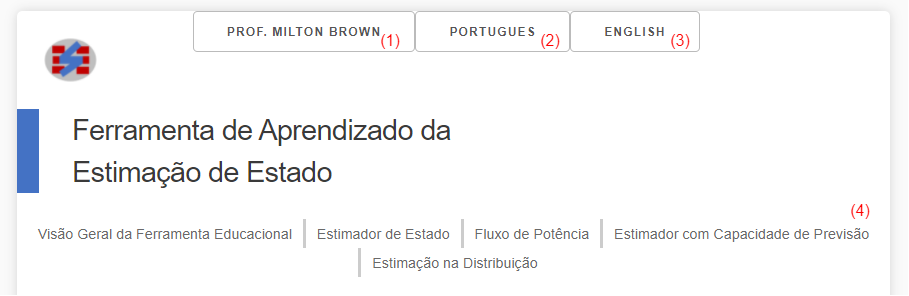
\includegraphics[scale=.4]{Imagens/Topo_pagina.png}
\caption{Opções de seleção de módulos da ESE}
\label{fig:opções_cabeçalio}
\end{figure}



A ferramenta foi dividida em módulos para proporcionar uma facilidade de uso e de desenvolvimento contínuo, conforme pode ser visto na Figura \ref{fig:opções_cabeçalio}. De maneira geral foram criados cinco módulos funcionais, sendo estes:
\begin{enumerate}
    \item \textbf{Visão Geral da Ferramenta:} Apresenta uma visão global da ferramenta, com uma breve descrição sobre utilidade da Estimação de Estado em sistemas elétricos de potência. Adicionalmente, são brevemente descritas as funcionalidades da ferramenta;
    \item \textbf{Estimação de Estado:} Função que recebe a topologia e parâmetros da rede, juntamente com um plano de medições e obtém o estado mais provável (módulo e ângulo das tensões nas barras). Nessa função também são realizadas as análises de observabilidade, criticalidade e a avaliação dos resíduos normalizados;
    \item \textbf{Fluxo de Potência:} Função que recebe os dados de topologia e parâmetros da rede, além dos dados das barras da rede (cargas). Os resultados desse fluxo de potência podem ser exportados como um arquivo de medidas para ser utilizado posteriormente na função de estimação;
    \item \textbf{Estimador de Estado com Capacidade de Previsão:}Fornecerá os valores previstos para o estado/medidas a serem usados para a construção de uma etapa de validação a priori (análise de inovações) dos valores de medidas recebidas para processamento;
    \item \textbf{Estimador de Estado na Distribuição:} Tratará o problema da estimação de estado em sistemas de distribuição com tratamento trifásico e diante da escassez de medidas;
\end{enumerate}


\section{Estimação de Estado}

O módulo \say{Estimador de Estado} necessita para sua execução  dois arquivos base. O primeiro deverá conter a topologia e os parâmetros da rede \textcolor{red}{(1)}, já o segundo, os valores das medições e seus respectivos desvios padrão. 
O usuário deverá selecionar \say{\textcolor{blue}{Arraste ou Selecione o Arquivo}} para carregar ambos os arquivos de seu repositório para a página da ferramenta. 
 A Figura \ref{fig:entrada_estimação} apresenta um exemplo da interface do programa quando são submetidas entradas referentes a um sistema de 3 barras (utilizado no decorrer deste tutorial).
 Em sequencia serão apresentados mais detalhes sobre a formatação dos arquivos.

\begin{figure}[H]
    \centering
    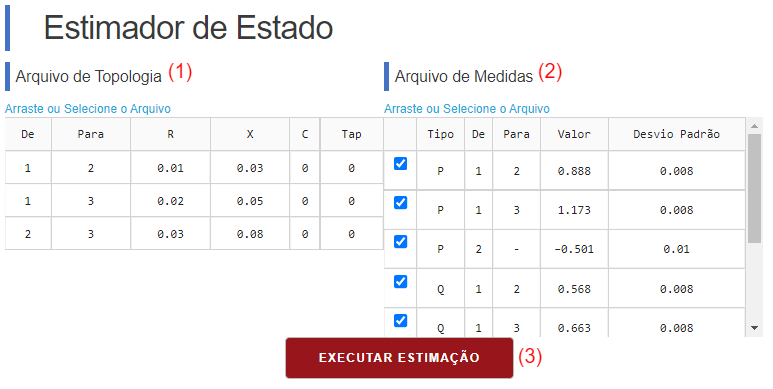
\includegraphics[scale=.45]{Imagens/Entradas_Estimação_de_Estado.png}
    \caption{Entradas do Módulo de Estimação de Estado}
    \label{fig:entrada_estimação}
\end{figure}

\subsection{Arquivo de Topologia}
O arquivo de topologia deve possuir extensão .xlsx e deve apresentar o cabeçalho de acordo com a Figura \ref{fig:arq_top}. As primeiras colunas (de e para) dizem respeito às extremidades das linhas de transmissão presentes na rede. A demais colunas informam os valores em p.u dos parâmetros das linhas, onde \say{R} significa resistência, \say{X} é a reatância, \say{C} é a capacitância \textit{shunt} completa da linha e por fim o \say{Tap} indica a relação de transformação no caso de transformadores.
\begin{figure}[H]
    \centering
    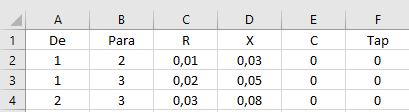
\includegraphics[scale=.7]{Imagens/Foto_Arquivo de_Topologia.JPG}
    \caption{Entradas do Módulo de Estimação de Estado}
    \label{fig:arq_top}
\end{figure}
\subsection{Arquivo de Medidas}
Esse arquivo também deve possuir a extensão .xlsx, além dos respectivos cabeçalhos apresentados na Figura \ref{fig:arq_meds}. A princípio, pode-se incluir no arquivo medidas de potência ativa (P), reativa (Q) e de módulo de tensão (V).
As colunas \say{De} e \say{Para} com valores indicam que a medida é de fluxo de potência. 
Caso seja uma medida de injeção  a terceira coluna deve possuir um traço, assim como no caso de medida de módulo de tensão. Por fim, as colunas \say{Valor} e \say{Desvio Padrão} correspondem aos valores em p.u das medidas e seus respectivos desvios.   
\begin{figure}[H]
    \centering
    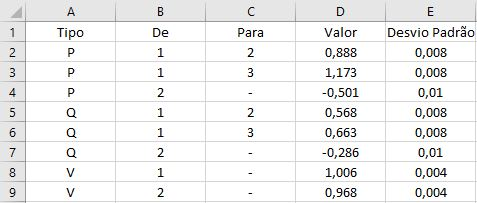
\includegraphics[scale=.7]{Imagens/Foto_Arquivo_de_Medidas.JPG}
    \caption{Entradas do Módulo de Estimação de Estado}
    \label{fig:arq_meds}
\end{figure}

\subsection{Botão de Estimação}
Com os arquivos carregados é indispensável que o usuário pressione o botão "Executar Estimação" para prosseguir com a utilização da ferramenta. Se tudo estiver correto, o processo seguirá e os resultados serão apresentados, caso contrário, o programa apresentará uma mensagem de alerta sobre não-observabilidade da rede, conforme a Figura \ref{fig:Pop_obs}. 

\begin{figure}[H]
    \centering
    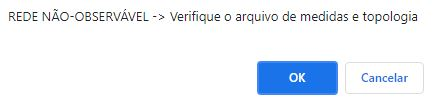
\includegraphics[scale = .7]{Imagens/Pop-up_Observabilidade.JPG}
    \caption{Mensagem de erro para rede não observável}
    \label{fig:Pop_obs}
\end{figure}

\subsection{Representação Topológica}
Após a inserção dos arquivos de topologia e das medidas, o ESE apresenta uma representação topológica da rede \textcolor{red}{(1)}, conforme a Figura \ref{fig::topology}. Além de proporcionar uma visão global da rede simulada é possível interagir com a figura da rede, com a possibilidade de movimentar as barras, reorganizar as linhas e aproximar a imagem para uma melhor visualização da rede.  

\begin{figure}[H]
    \centering
    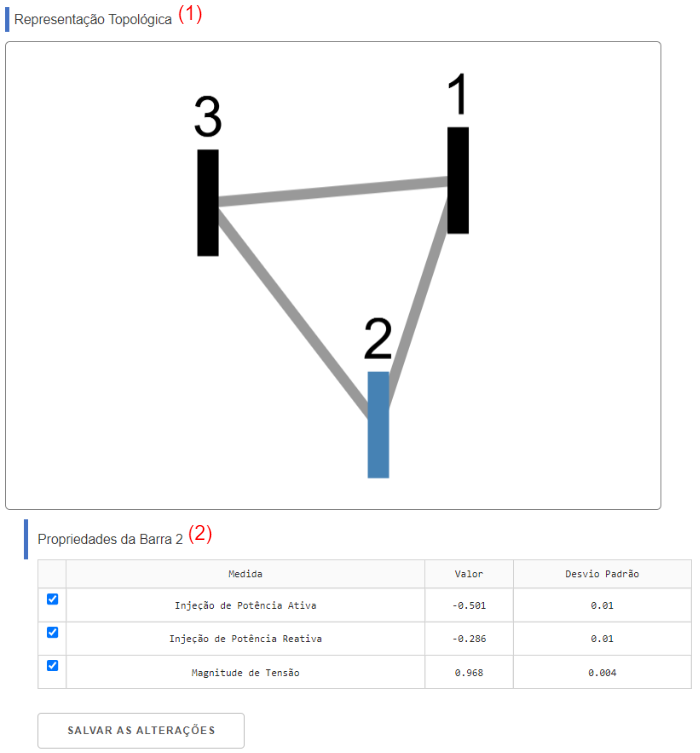
\includegraphics[scale = .47]{Imagens/Representação_Topologica.png}
    \caption{Representação topológica.}
    \label{fig::topology}
\end{figure}

Clicar nos elementos das redes (barras ou linhas) resultará na mudança de cor do item selecionado, destacando-o dos demais. Esta seleção também habilitará uma tabela editável \textcolor{red}{(2)} que contém as medidas presentes no elemento, que permitirá mudanças nos seus valores, além de novas inserções. Essas possibilidades serão abordadas nas seções subsequentes. 

\subsection{Análise de Criticalidades}
Após o usuário clicar em \say{Executar Estimação}, a ferramenta é capaz de identificar as medidas e duplas críticas presentes no plano de medição. Em relação às duplas críticas, aquelas que fazem parte de um mesmo conjunto crítico são destacadas com uma mesma cor. Por fim, é possível exportar esse resultado clicando-se no botão \say{Export}.

\begin{figure}[H]
    \centering
    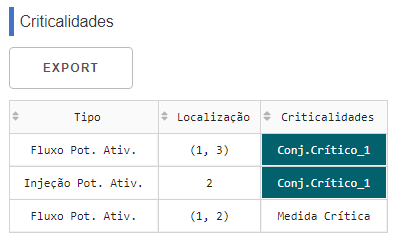
\includegraphics[scale = .65]{Imagens/Criticalidades_Ferrameta.PNG}
    \caption{Resultado de Criticalidade}
    \label{fig:my_label}
\end{figure}


\subsection{Gráfico da Função Objetivo J(x)}
O programa apresenta a trajetória de convergência do método de Newton-Raphson, Figura \ref{fig:fobj} . Vale salientar que considera-se os \say{logaritmos} de $J(x)$ para facilitar a representação gráfica. Além disso, pode-se exportar o gráfico como imagem ou manipulá-lo para destacar regiões, etc.

\begin{figure}[H]
    \centering
    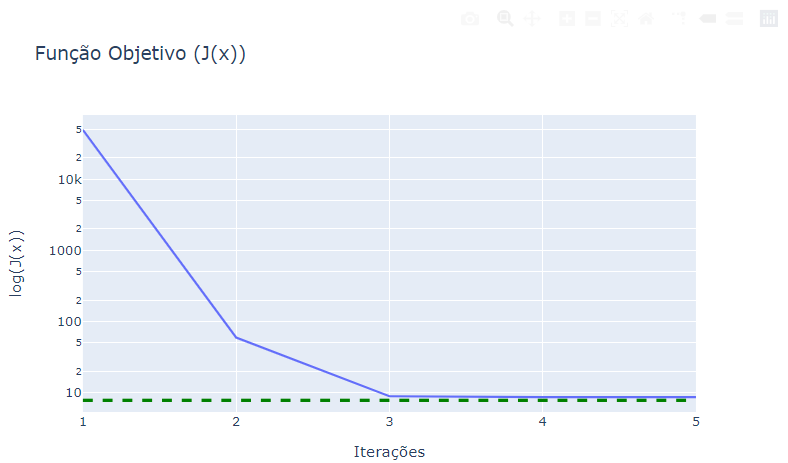
\includegraphics[scale=.5]{Imagens/Função_Objetivo_Ferramenta.PNG}
    \caption{Função Objetivo.}
    \label{fig:fobj}
\end{figure}

\subsection{Resultado da Estimação}
A tabela representada pela Figura \ref{fig:results_SE} indica os módulos e ângulos das tensões nos barramentos da rede obtidos pelo processo de Estimação de Estado. Vale ressaltar que os valores de magnitude das tensões estão em p.u e os de ângulo em graus. Assim como nas tabelas anteriores é possível exportar os resultados.  
\begin{figure}[H]
    \centering
    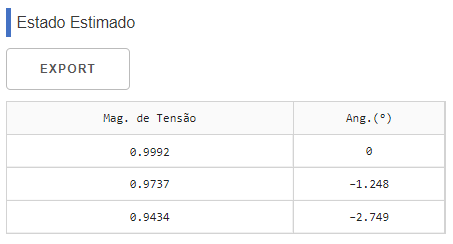
\includegraphics[scale = .65]{Imagens/Medidas_Estimadas_Ferramenta.PNG}
    \caption{Estado Estimado}
    \label{fig:results_SE}
\end{figure}


\subsection{Análise de Resíduos}
Com o estado estimado o programa constrói a tabela representada na Figura \ref{fig:meds_filters}, que apresenta os valores das medidas juntamente com seus valores estimados. Adicionalmente são calculados os desvios e os resíduos normalizados para cada uma das medições. No caso de medidas críticas os resíduos não devem ser normalizados e por isso não são representados, além disso os maiores resíduos que 3 são destacados par alertar o usuário no caso de possíveis erros grosseiros. Mais detalhes sobre esse ponto serão apresentados nas seções vindouras.
\begin{figure}[H]
    \centering
    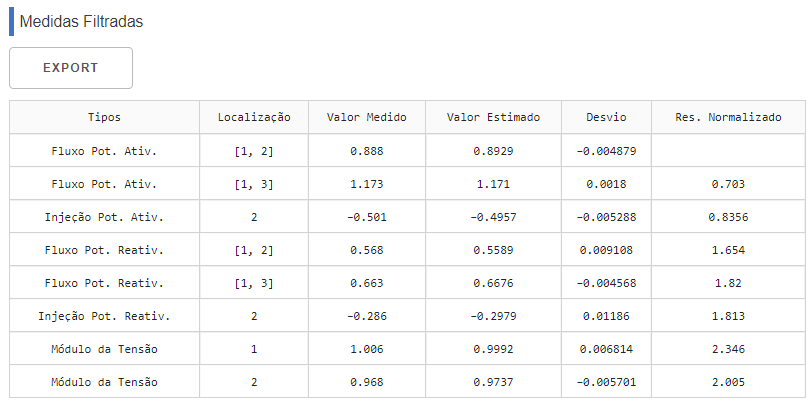
\includegraphics[scale = .5]{Imagens/Residuos_Normalizados_Ferramenta.PNG}
    \caption{Medidas Filtradas}
    \label{fig:meds_filters}
\end{figure}

\subsection{Adição, Remoção e Alteração de Dados de Entrada}
Caso o usuário deseje realizar simulações de eventos que alterem o plano de medição (ex: desligamento, alteração dos valores, inserção de erros, etc) a ferramenta possui flexibilidade para tal. O caso exemplo na sequência descreve todas as possibilidades.

\subsubsection{Desligamento das Medidas}
Seja o caso base de 3 barras apresentado anteriormente, supondo que o usuário deseje desligar medida a medida $P_{1-3}$. Utilizando a Ferramenta Educacional esta ação pode ser realizada através da caixa de seleção da tabela referente ao arquivo de medidas, como está ilustrado na figura \ref{fig:remov_med}. 


\begin{figure}[H]
    \centering
    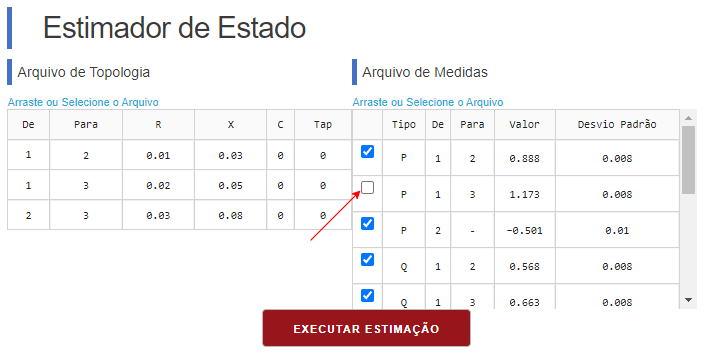
\includegraphics[scale=.5]{Imagens/Remoção_de_medidas.PNG}
    \caption{Remoção de medidas pelo arquivo de entrada}
    \label{fig:remov_med}
\end{figure}

A Remoção de medidas também pode ser realizada na interface da topologia da rede. Para isso, o usuário precisa selecionar o elemento da rede onde encontra-se a medida e, na sequência, desmarcar a opção da caixa de seleção referente à medida desejada. A figura \ref{fig:remov_med_top} ilustra a remoção da medida $P_{1-3}$ (fluxo ativo do ramo [1-3]) através da interface topológica.
Esta opção de remoção torna-se vantajosa para redes de maior porte, onde um foco em regiões da rede pode ser desejado.

\begin{figure}[H]
    \centering
    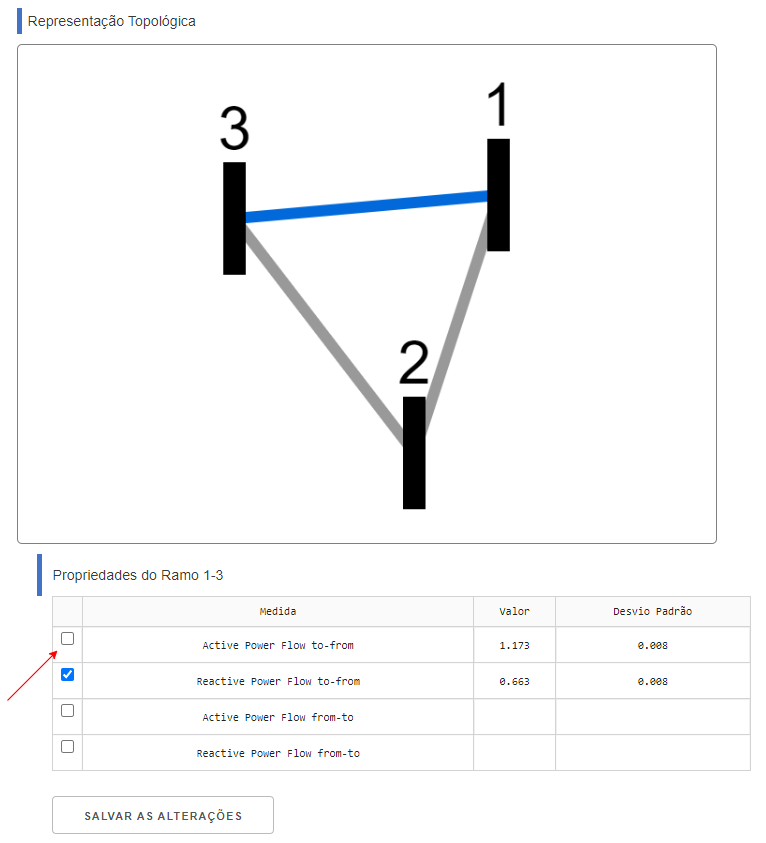
\includegraphics[scale=.45]{Imagens/Remoção_de_medidas_Topologia.PNG}
    \caption{Remoção de medidas pela opção interface da topologia da rede}
    \label{fig:remov_med_top}
\end{figure}



\subsubsection{Adição de Novas Medidas}
Caso o usuário deseje inserir novas medições existem duas possibilidades. A primeira delas é alterar o arquivo de medidas e recarregá-lo na ferramenta. Essa opção é mais trabalhosa e é indicada quando muitas inserções serão realizadas. Em contrapartida, quando deseja-se inserir um pequeno conjunto de medidas é possível fazer uso da representação topológica. Para tal o usuário deve clicar nas barras ou linhas em que se deseja inserir as novas medidas \textcolor{red}{(1)}. Após clicar na caixa de seleção, e adicionar o valor e o desvio padrão desejados \textcolor{red}{(2)}, é indispensável que o usuário clique em "Salvar Alterações" \textcolor{red}{(3)}. Como pode ser visto na Figura \ref{fig:add_val_confirm}, a inserção pode ser conferida observando-se a tabela de medidas \textcolor{red}{(4)}.  

\begin{figure}[H]
    \centering
    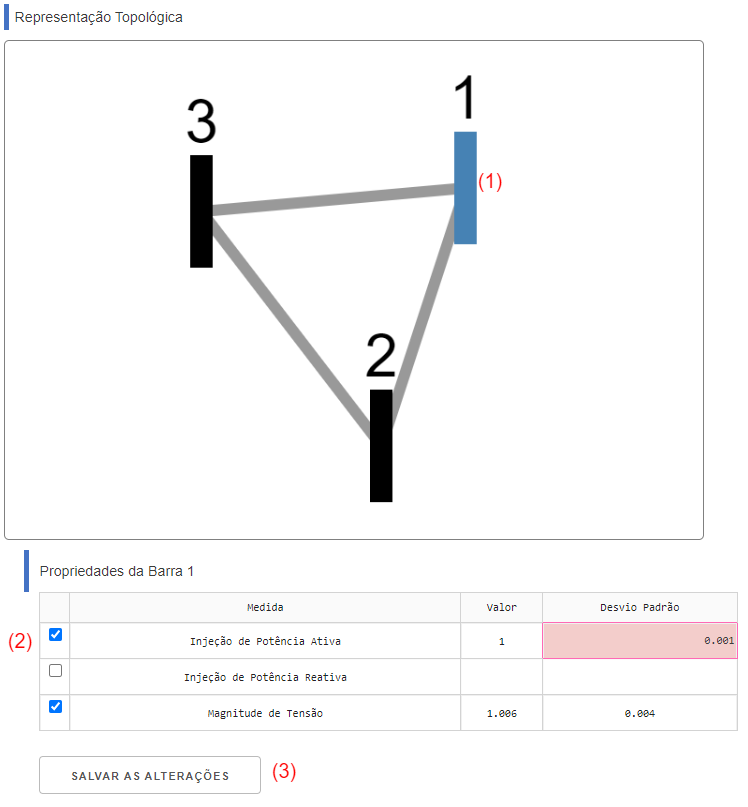
\includegraphics[scale=.45]{Imagens/Adição_de_medidas.png}
    \caption{Adição de medidas no plano de medição pela interface topológica}
    \label{fig:add_val}
\end{figure}

\begin{figure}[H]
    \centering
    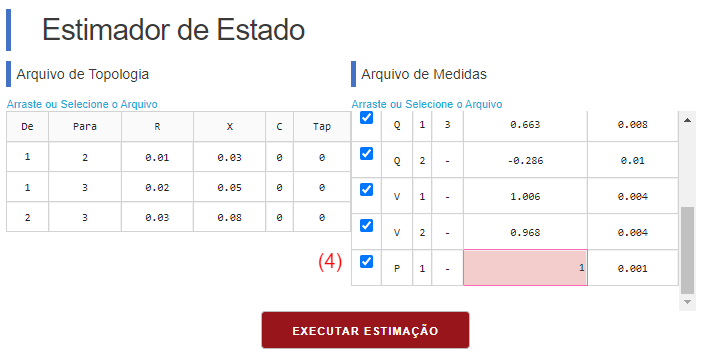
\includegraphics[scale=.45]{Imagens/Confirmação_Adição_de_medidas.png}
    \caption{Valor alterado na Tabela de entrada de medidas}
    \label{fig:add_val_confirm}
\end{figure}

\subsubsection{Alteração de Valores}
Suponhamos agora que se deseje realizar a alteração de grandezas do arquivo de medidas. Nesse caso não há a necessidade de alterar o arquivo base, mas basta o usuário clicar na célula (ou células) que se deseja alterar, digitar o novo valor e \textbf{pressionar a tecla "ENTER"} para confirmar a alteração. Destaca-se que é necessário, sempre que houver modificações, que o usuário \textbf{clique no botão "EXECUTAR ESTIMAÇÃO"}.



\begin{figure}[H]
    \centering
    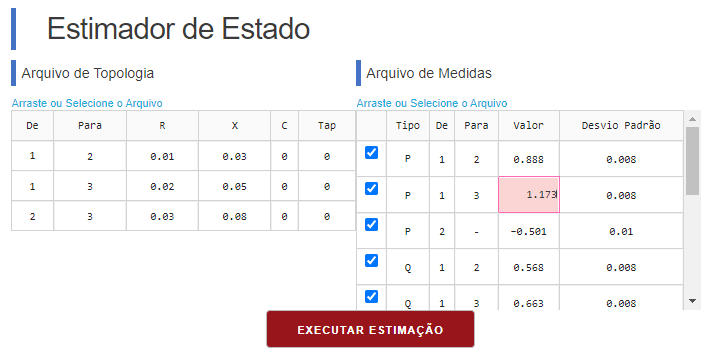
\includegraphics[scale=.70]{Imagens/Alteração_de_valor.PNG}
    \caption{Alteração de valores diretamente na tabela de entrada}
    \label{fig:alt_vaç}
\end{figure}

Adicionalmente, para sistemas de maiores dimensões, pode-se desejar alterar medidas de regiões específicas da rede. Para tal é possível utilizar o grafo da rede e clicando-se nos elementos deste alterar os valores na tabela que surgirá após o clique. Essa situação está representada na Fig. \ref{fig:alt_top}. 

\begin{figure}[H]
    \centering
    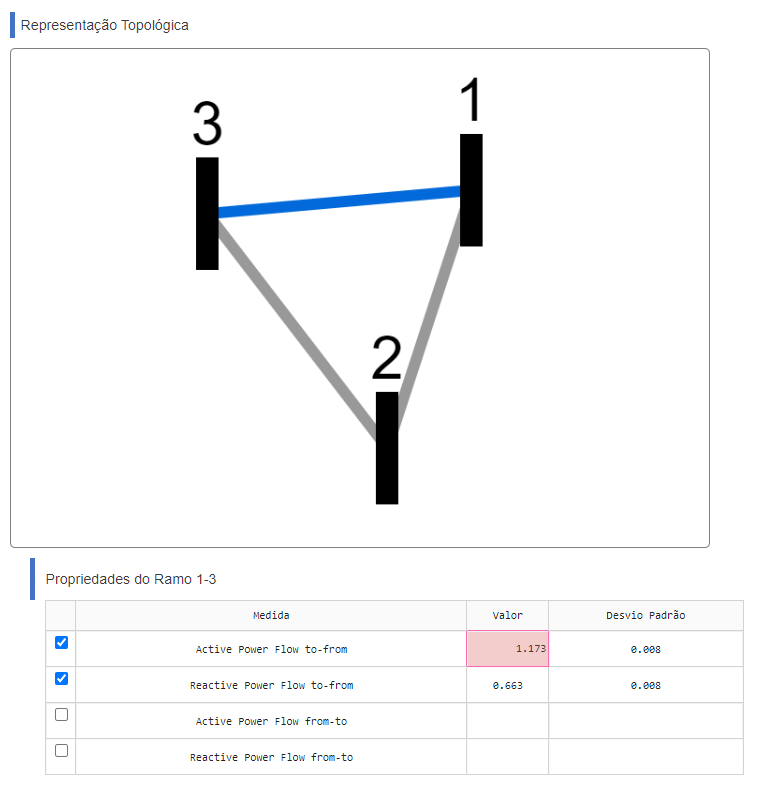
\includegraphics[scale = .7]{Imagens/Alteração_pelo_Grafo.PNG}
    \caption{Alteração de valores na topologia da rede}
    \label{fig:alt_top}
\end{figure}


\section{Fluxo de Potência}

\section{Estimador com Capacidade de Previsão}

\section{Estimador na Distribuição}


\end{document}
